\documentclass{beamer}
\usetheme{Boadilla}

\usepackage{amsmath}
\usepackage{amsfonts}
\usepackage{hyperref}
\usepackage{multicol}

\usepackage{amsmath}
\DeclareMathOperator*{\argmax}{arg\,max}
\DeclareMathOperator*{\argmin}{arg\,min}

\newcommand{\bz}{\mathbf{z}}
\newcommand{\bx}{\mathbf{x}}
\newcommand{\by}{\mathbf{y}}
\newcommand{\bv}{\mathbf{v}}
\newcommand{\bw}{\mathbf{w}}
\newcommand{\ba}{\mathbf{a}}
\newcommand{\bb}{\mathbf{b}}
\newcommand{\bff}{\mathbf{f}}
\newcommand{\bh}{\mathbf{h}}
\newcommand{\bl}{\mathbf{l}}
\newcommand{\bp}{\mathbf{p}}
\newcommand{\bq}{\mathbf{q}}
\newcommand{\bs}{\mathbf{s}}
\newcommand{\bt}{\mathbf{t}}
\newcommand{\bu}{\mathbf{u}}
\newcommand{\bT}{\mathbf{T}}
\newcommand{\bX}{\mathbf{X}}
\newcommand{\bZ}{\mathbf{Z}}
\newcommand{\bS}{\mathbf{S}}
\newcommand{\bH}{\mathbf{H}}
\newcommand{\bW}{\mathbf{W}}
\newcommand{\bY}{\mathbf{Y}}
\newcommand{\bU}{\mathbf{U}}
\newcommand{\bQ}{\mathbf{Q}}
\newcommand{\bP}{\mathbf{P}}
\newcommand{\bA}{\mathbf{A}}
\newcommand{\bB}{\mathbf{B}}
\newcommand{\bC}{\mathbf{C}}
\newcommand{\bE}{\mathbf{E}}
\newcommand{\bF}{\mathbf{F}}
\newcommand{\bsigma}{\boldsymbol{\sigma}}
\newcommand{\bomega}{\boldsymbol{\omega}}
\newcommand{\btheta}{\boldsymbol{\theta}}
\newcommand{\bgamma}{\boldsymbol{\gamma}}
\newcommand{\bdelta}{\boldsymbol{\delta}}
\newcommand{\bPsi}{\boldsymbol{\Psi}}
\newcommand{\bpsi}{\boldsymbol{\psi}}
\newcommand{\bxi}{\boldsymbol{\xi}}
\newcommand{\bmu}{\boldsymbol{\mu}}
\newcommand{\bchi}{\boldsymbol{\chi}}
\newcommand{\bzeta}{\boldsymbol{\zeta}}
\newcommand{\blambda}{\boldsymbol{\lambda}}
\newcommand{\beps}{\boldsymbol{\varepsilon}}
\newcommand{\bZeta}{\boldsymbol{Z}}
\newcommand{\dH}{\mathds{H}}
\newcommand{\dR}{\mathds{R}}

\title{Discovering Inductive Bias with Gibbs Priors}
\author{Eduard Vladimirov}
\institute{MIPT, 2023}


\begin{document}
	
	\begin{frame}
		\titlepage
	\end{frame}
	
	
	\begin{frame}
		\tableofcontents
	\end{frame}
	
	
	\section{Motivation \& Background}
	\begin{frame}{Motivation}
		\begin{block}{Main idea}
			The problem: diagnosing approximate Bayesian inference methods in terms
			of their inductive bias
			
			The solution: Gibbs prior as a natural solution
			to the problem and as a diagnostic tool. It is based on pseudo-Gibbs sampling
		\end{block}
	
		\begin{figure}[bhtp]
			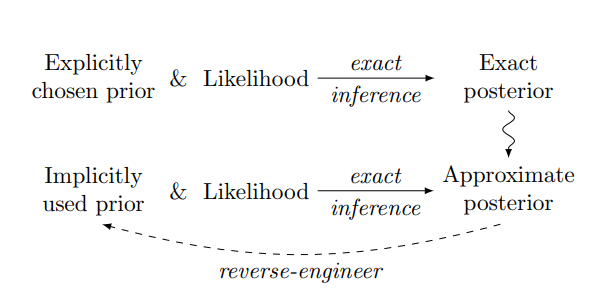
\includegraphics[width=\linewidth]{main-idea.png}
			\caption{Main Idea}
		\end{figure}
	\end{frame}
	
	
	\begin{frame}{Background}
		\begin{figure}[bhtp]
			
\includegraphics[width=0.6\linewidth]{mcmc.png}
			\caption{Markov Chain Monte-Carlo}
		\end{figure}
	
		\begin{figure}[bhtp]
			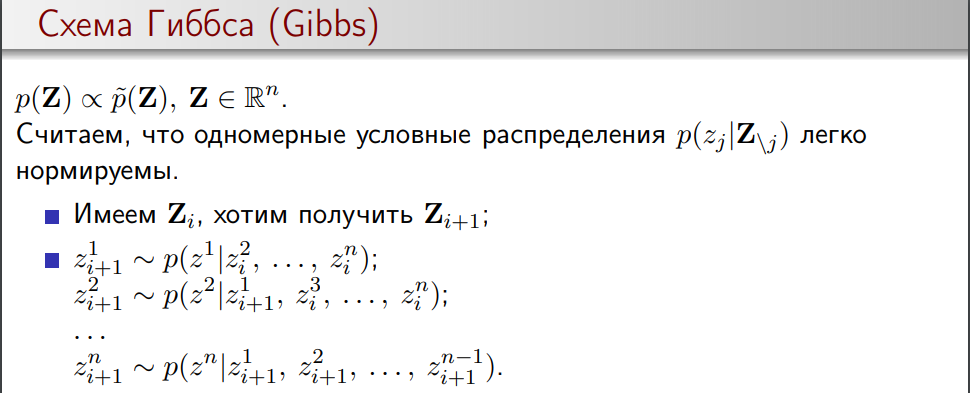
\includegraphics[width=0.6\linewidth]{gibbs-chain.png}
			\caption{Gibbs schema}
		\end{figure}
	\end{frame}

	\begin{frame}{Existing approaches}
		\begin{table}[bhtp]
			\centering
			\begin{tabular}{|p{0.45\textwidth}|p{0.45\textwidth}|}
				\hline
				\textbf{Divergence-based Diagnostics} & \textbf{True Posterior-based Diagnostics} \\
				\hline
				Stein discrepancies between the posterior and its approximation. & distortion map for posterior cumulative distribution functions to the identity. \\
				symmetric KL divergence between the approximation and another baseline approximation. & compare average posterior means and covariances to prior means and covariances. \\
				the symmetric KL divergence between the true joint distribution \( p(y)p(\theta|y) \) and its approximation \( p(y)q(\theta|y) \). & distribution of posterior quantiles, tested for uniformity; corrected by Talts et al. (2018). \\
				& test for uniformity of p-values related to the coverage property; this method is extended by Rodrigues et al. (2018). \\
				\hline
			\end{tabular}
			\caption{Categorization of diagnostics in literature}
		\end{table}
	\end{frame}
	
	
	\section{Theory}
	\begin{frame}{Designation and pointwise-prior}
		Let \( (f(\cdot|\theta)) \) be the likelihood and \( (q(\cdot|y)) \) the approximations to the posteriors \( (p(\cdot|y)) \). It is reasonable to define the implicit prior to the approximations by fixing an observation \( y \) and simply reverting Bayes' theorem
		\[ \pi_y(\theta) \propto q(\theta|y)/f(y|\theta). \]
		Unfortunately, \( \pi_y \) generally depends on the observation \( y \). This means that the approximations to different observations can correspond to different implicit priors, in which case no single distribution \( \tilde{\pi} \) satisfies \( q(\theta|y) \propto \tilde{\pi}(\theta)f(y|\theta) \).
	\end{frame}
	
	
	\begin{frame}{Gibbs prior}
		
	\begin{block}{Definition}
		For two families of distributions \( (f(\cdot|\theta))_{\theta \in \Theta} \) on \( \mathcal{Y} \) and \( (q(\cdot|y))_{y \in \mathcal{Y}} \) on \( \Theta \) consider the discrete-time Markov chain on \( \Theta \) whose transition function is given by
		\[ r(\theta'|\theta) = \mathbb{E}_{Y \sim f(\cdot)}[q(\theta'|Y)]. \]
		This chain is called the \textit{Gibbs chain}. Any stationary distribution of this Markov chain is called a \textit{Gibbs prior} and denoted by \( \pi_G \).
	\end{block}

	\begin{multicols}{2}
		\begin{figure}[bhtp]
			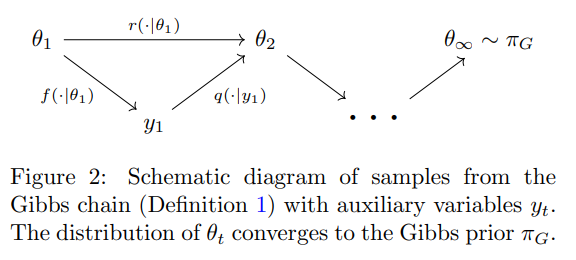
\includegraphics[width=\linewidth]{sampling-schema.png}
			\caption{Sampling from Gibbs chain}
		\end{figure}
		
		\begin{figure}[bhtp]
			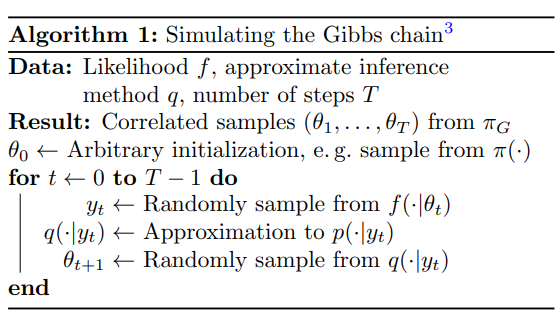
\includegraphics[width=\linewidth]{algo.png}
			\caption{Simulating the Gibbs chain}
		\end{figure}
	\end{multicols}	
	\end{frame}
	
	\begin{frame}{Existence and uniqueness of Gibbs priors}
		\begin{block}{Theorem}
			Consider two families of distributions \( F = (f(\cdot|\theta))_{\theta \in \Theta} \) on \( \mathcal{Y} \) and \( Q = (q(\cdot|y))_{y \in \mathcal{Y}} \) on \( \Theta \). Let \( M \) be the corresponding Gibbs chain.
			
			\begin{itemize}
				\item[(i)] If \( F \) and \( Q \) are compatible with joint distribution \( p(\theta, y) \), then the marginal \( p(\theta) \) is a Gibbs prior. If \( M \) is additionally irreducible, then it is the only Gibbs prior.
				\item[(ii)] If \( \Theta \) and \( \mathcal{Y} \) are finite, then there exists a Gibbs prior. If additionally \( F \) or \( Q \) are positive, then the Gibbs prior is unique.
			\end{itemize}
		\end{block}
	\end{frame}
	
	\section{Computation experiment}
	
	\begin{frame}{Gaussian Toy Model}
		\textbf{Problem}: estimate the mean \( \theta \in \mathbb{R}^d \) of a \( d \)-dimensional Gaussian distribution with known covariance matrix based on \( n \) independent samples \( y_1, \ldots, y_n \in \mathbb{R}^d \). Placing a Gaussian prior on \( \theta \) yields the Bayesian model
		\[
		\theta \sim \mathcal{N}(\mu_0, \Sigma_0),
		\]
		\[
		y_i|\theta \overset{\text{indep}}{\sim} \mathcal{N}(\theta, \Sigma), \quad i = 1, \ldots, n,
		\]
		where \( \mu_0 \in \mathbb{R}^d \) and \( \Sigma_0, \Sigma \in \mathbb{R}^{d \times d} \) are positive definite.
	\end{frame}


	\begin{frame}{Gaussian Toy Model}
		\begin{figure}[bhtp]
			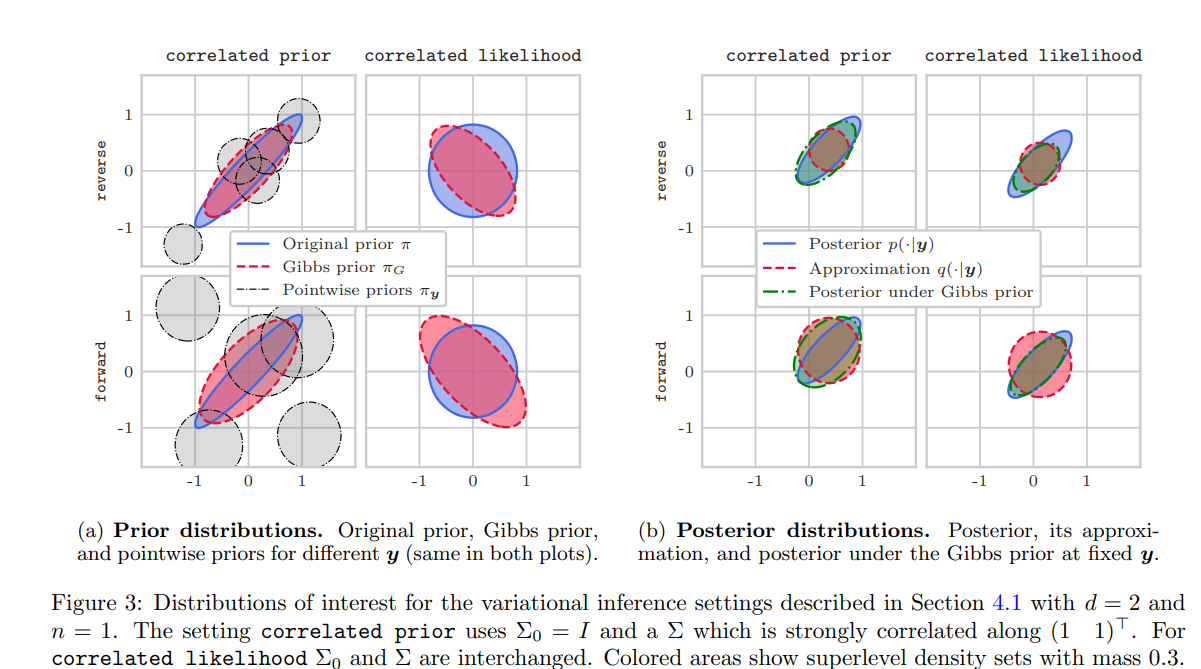
\includegraphics[width=\linewidth]{gaussian-toy-example.png}
			\caption{Prior and posterior distributions}
		\end{figure}
	\end{frame}

	
	\begin{frame}{Baseline}
		This diagnostic is based on the stationarity equation of the prior \( \pi \) under the Gibbs chain, but only considers 1-step transitions with some test statistics \( f: \Theta \to \mathbb{R} \). Under random samples \( \tilde{\theta} \sim \pi, \tilde{y} \sim f(\cdot|\tilde{\theta}), \) and \( \theta_1, \ldots, \theta_L \sim q(\cdot|\tilde{y}), \) the rank of \( f(\tilde{\theta}) \) in \( \{f(\theta_1), \ldots, f(\theta_L)\} \) is computed. This is repeated over multiple draws of \( (\tilde{\theta}, \tilde{y}), \) which gives a histogram of the ranks. Since the histogram is uniform under the exact posterior, any deviations from uniformity indicate an approximation mismatch.
		
		
		\begin{figure}[bhtp]
			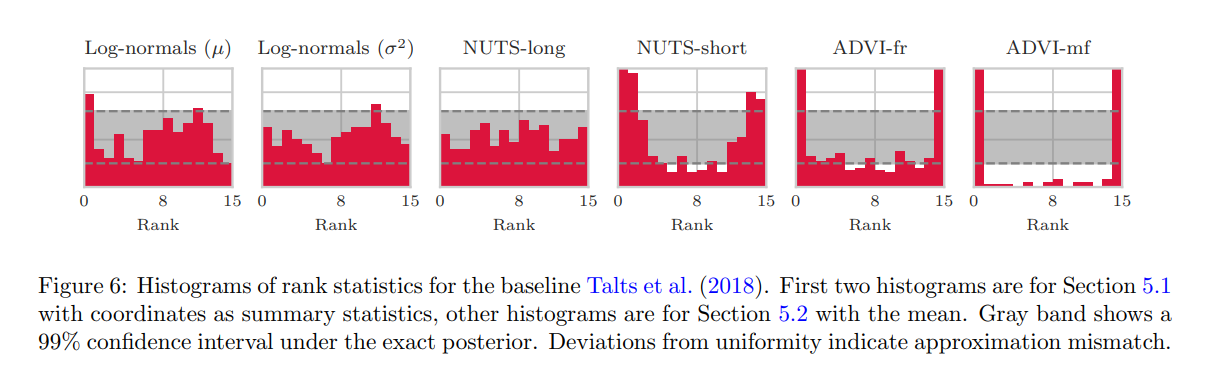
\includegraphics[width=\linewidth]{baseline-images.png}
			\caption{Baseline}
		\end{figure}
	\end{frame}


	\begin{frame}{Sum of Log-Normals}
		\textbf{Setup}: The model describes the sum of \( L = 10 \) independent samples from a log-normal distribution and is given by
		
		\[
		\mu \sim \mathcal{N}(0, 1), \quad \sigma^2 \sim \text{Gamma}(1, 1),
		\]
		
		\[
		x_l|\theta = (\mu, \sigma^2) \overset{\text{indep}}{\sim} \text{LogNormal}(\mu, \sigma^2), \quad y = \sum_{l=1}^{L} x_l.
		\]
		
		\begin{figure}[bhtp]
			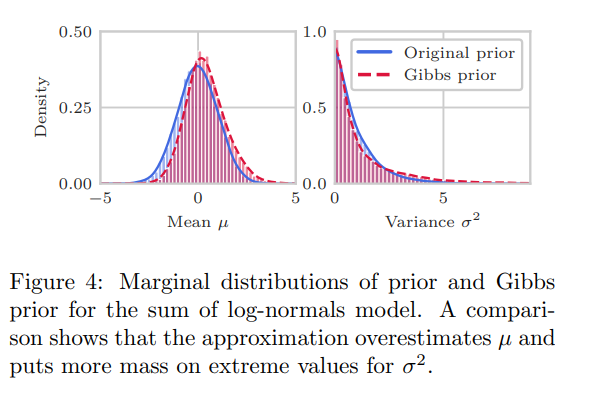
\includegraphics[width=0.8\linewidth]{sum-log-normals.png}
			\caption{Sum of Log-Normals}
		\end{figure}
	\end{frame}


	\begin{frame}{Stochastic Volatility}
		\textbf{Setup}: Stochastic volatility models are used in mathematical finance for time series to describe the latent variation of trading price (called the returns). We consider a model similar to Hoffman and Gelman (2014):
		
		\[
		\theta_i|\theta_{i-1} \sim \mathcal{N}(\theta_i, \sigma^2), \quad i = 1, \ldots, T,
		\]
		
		\[
		y_i \overset{\text{indep}}{\sim} \text{StudentT}(\nu, 0, \exp(\theta_i)), \quad i = 1, \ldots, T,
		\]
		
		
		\begin{figure}[bhtp]
			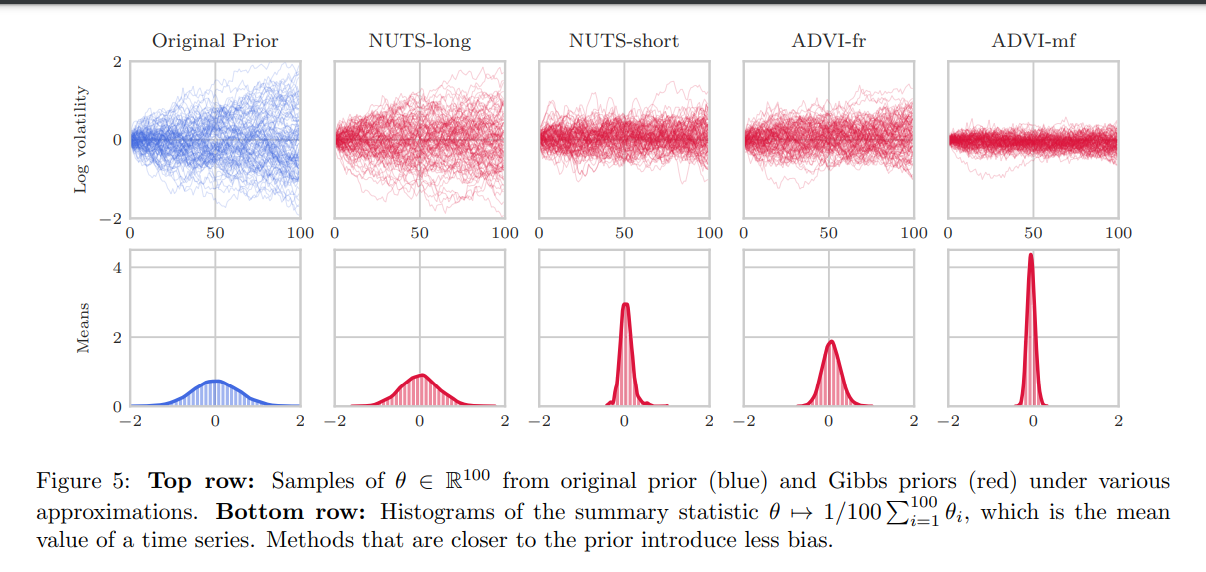
\includegraphics[width=0.8\linewidth]{stochastic-volatility.png}
			\caption{Stochastic Volatility}
		\end{figure}
	\end{frame}
	
	
	\begin{frame}{Literature}
		\begin{enumerate}
			\item \textbf{Main article} \href{https://arxiv.org/pdf/2203.03353.pdf}
			{Discovering Inductive Bias with Gibbs Priors: A Diagnostic Tool for Approximate Bayesian Inference}.
		\end{enumerate}
	\end{frame}
	
	
	
\end{document}